\section{Introduction}

    \begin{frame}{Introduction: main features}
        \begin{columns}[t, onlytextwidth]
            \column{0.33\textwidth}
            \centering
            
\includegraphics[height=1.5cm, keepaspectratio]{images/shapes.pdf}

            \textbf{General purpose}

            \column{0.33\textwidth}
            \centering
            
\includegraphics[height=1.5cm, keepaspectratio]{images/fast.pdf}
            
            \textbf{Blazingly fast}

            \column{0.33\textwidth}
            \centering
            
\includegraphics[height=1.5cm, keepaspectratio]{images/memory.pdf}
            
            \textbf{Memory safe}
        \end{columns}

        \vspace{1cm}

        \begin{columns}[t, onlytextwidth]
            \column{0.5\textwidth}
            \centering
            
\includegraphics[height=1.5cm, keepaspectratio]{images/no-gc.pdf}

            \textbf{No Garbage Collector}

            \column{0.5\textwidth}
            \centering
            
\includegraphics[height=1.5cm, keepaspectratio]{images/toolbox.pdf}

            \textbf{Tools} \\ (doc, cargo, libraries)
        \end{columns}
    \end{frame}

    \begin{frame}{Introduction: history}
        \begin{vtimeline}[description={text width=7cm},
        row sep=4ex]
        2006 & Mozilla creates Rust for the Servo's project \endlr
        2010 & Rust is announced at Mozilla Summit\endlr
        2012 & Alpha release\endlr
        2013 & Version 0.6 release\endlr
        2015 & First stable release (Rust 1.0)\endlr
        2021 & The Rust Foundation is founded\endlr
    \end{vtimeline}
    \end{frame}

    \begin{frame}{Introduction: who uses it?}
        \begin{itemize}
            \item AWS: Firecracker powers Lambda and Fargate
            \item Google: parts of the Fuschia operating system
            \item Linux: 2nd official language for the Kernel!
            \item CloudFlare: quic / http 3 implementation
            \item Dropbox: file storage
            \item Clever Cloud: reverse proxy
            \item Atlassian, Canonical, Coursera, Chef, Deliveroo, NPM, Sentry...
            \item Growing ecosystem for embedded development
        \end{itemize}
    \end{frame}

    \begin{frame}{Introduction: Rust vs C/C++}
        \begin{center}
            \begin{tabular}{ |c|c|c|c| } 
             \hline
             \textbf{Properties} & \textbf{Rust} & \textbf{C} & \textbf{C++} \\
             \hline
             Type safety & Safe & Unsafe & Unsafe \\
             \hline
             Type expression & Implicit/Explicit & Explicit & Explicit \\
             \hline
             Type checking & Static/dynamic & Static & Static \\
             \hline
             Garbage collector & No & No & No \\
             \hline
            \end{tabular}
            \end{center}
    \end{frame}
    

    \begin{frame}{Introduction: learning Rust}
        \begin{columns}[t, onlytextwidth]
            \column{0.5\textwidth}
            \centering
            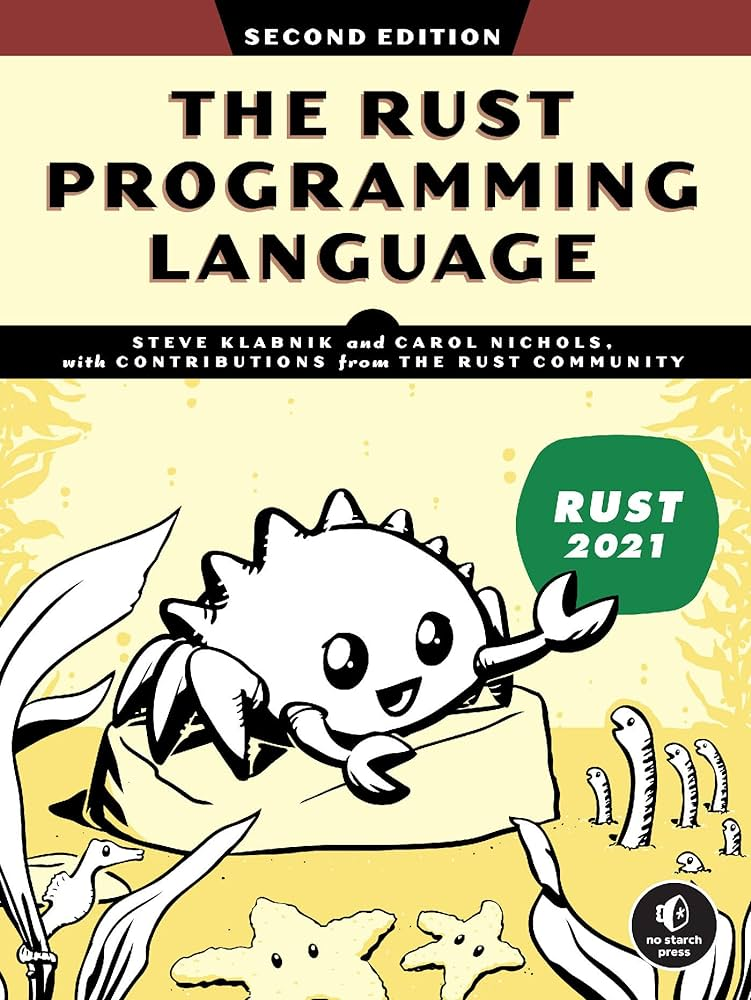
\includegraphics[height=5.5cm, keepaspectratio]{images/rust-book.jpg}

            \small Online at https://www.rust-lang.org

            \column{0.5\textwidth}
            \centering
            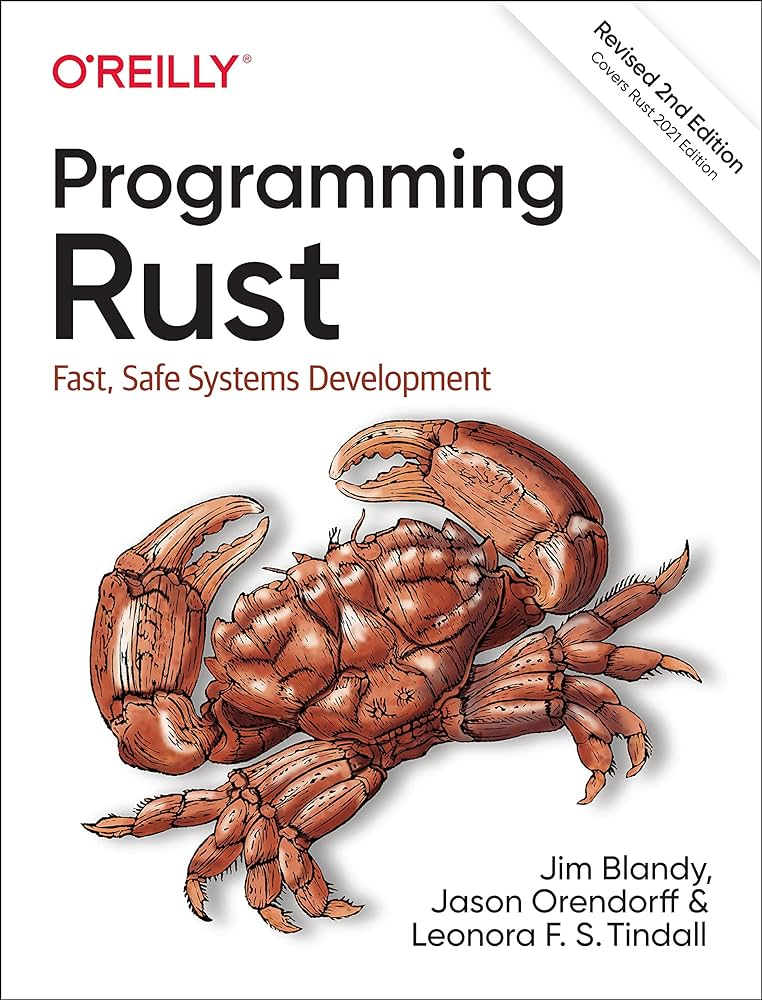
\includegraphics[height=5.5cm, keepaspectratio]{images/programming-rust.jpg}
        \end{columns}
    \end{frame}

    \begin{frame}[containsverbatim]{Getting started}
        \small
        \begin{block}{Installing on MacOS/Unix}
            \tt{curl --proto '=https' --tlsv1.2 -sSf https://sh.rustup.rs | sh}
        \end{block}

        \begin{block}{Installing on Windows}
            Download and install the \tt{rustup-init.exe} from the official website. 
        \end{block}

        \begin{alertblock}{Verifying the installation}
            \tt{rustc --version}
        \end{alertblock}
    \end{frame}